\documentclass{article}
\usepackage{amsmath}
\usepackage{amssymb}
\usepackage{graphicx}
\usepackage{subcaption}
\usepackage[utf8]{inputenc}
\usepackage[table]{xcolor}
\usepackage[margin=1.2in]{geometry}


\usepackage{lipsum}

\title{Statistical Mean Reversion of \\
Airline and Oil Company Stock Prices \\
\large CSC 265 Final Project}
\author{Dominick Harasimiuk - 30702462\\
Source Code Available At:\\ 
https://github.com/DominickH20/statistical-mean-reversion}
\date{May 7, 2021}


\begin{document}
\maketitle

\vspace{1cm}

\begin{abstract}
\noindent
This paper demonstrates the development and analysis of two forms of statistical
mean reversion (statistical arbitrage) strategies for trading airline and oil company
stocks. The first strategy is a pairwise model that leverages correlations among
pairs of stocks to trade. It is fit using OLS and performs rather well out of sample.
The second strategy is a basket model that leverages correlations among baskets of 
securities. To handle the multicollinearity problem within a basket, a principal component
decomposition is applied to the data before fitting with OLS. The basket strategy suffers 
from higher
volatility and noise in the signal, but still demonstrates the presence of a signal. 
The deterioration found in the basket strategy relative to the pairwise strategy is likely
attributable to the higher dimensionality of the data and distributional nuances in the
data that prohibit effective feature selection. 
\end{abstract}

\newpage
\section{Introduction}
The intent of this paper is to showcase a reliable statistical mean reversion trading strategy
on correlated baskets of stocks, specifically airline and oil company stocks. Airline companies
are exposed to very similar pools of risk, and the same can be said for oil companies. Because
of this, one would expect their stock prices to move together when these underlying risk
factors change. Because airlines are large consumers of oil, one might expect the airline and
oil sectors to exhibit some relationship as well.
\subsection{Statistical Mean Reversion}
This paper aims to develop a model for how these companies behave in relation
to one another. This model can be thought of as the "mean" in this mean reversion concept. I
utilize this model in the context of a trading strategy by computing the expected stock return 
at time $t$, call it $e_t$. The expected return can be compared to the actual return, $a_t$
at that same time period $t$. This generates a residual, $r_t = a_t - e_t$. If this residual
is sufficiently positive, then the strategy concludes that the stock in question has grown too 
much over the period, so it would sell. Likewise, if the $r_t$ is sufficiently negative, then the 
strategy judges that stock has underperformed over the period relative to its peers, so it would buy. In both cases
the strategy is betting on convergence to the statistical relationship between the securities.
In this paper, I outline such strategies on pairs of securities as well as baskets of securities,
using principal component analysis to handle the multicollinearity problem for regression
models implemented on such data.

\subsection{Data}
\subsubsection{Scope}
The data used in the subsequent analyses were obtained from the Alpaca Markets historical 
market data API. The securities examined in this study are the following: American Airlines
(AAL), Delta Airlines (DAL), Southwest Airlines (LUV), Allegiant Airlines (ALGT), United
Airlines (UAL), Chevron (CVX), Marathon Oil (MRO), Murphy Oil (MUR), Exxon Mobil (XOM),
Devon Energy (DVN), SPDR S\&P 500 ETF, and iShares Treasury Bond ETF (TLT). There 
are 5 airline companies, 5 oil companies, and 2 market factors (SPY and TLT). The motivation
behind including the market factors in this study is that they help parameterize what is going
on in equity and debt markets at any given point in time.
The data range from January 1st
2016 to May 1st 2021. The years 2020 and 2021 are held out as test data while the
rest of the data is used to train the models. Given the occurrence of the pandemic in 2020,
this is a particularly challenging test set. 
\subsubsection{Data Format}
The data is organized in a \textit{bar} format.
Bars are a common way of aggregating financial data and are structured as follows:
$$B_{S} = \begin{bmatrix} \mathrm{bar}_0, & \mathrm{bar}_1, & 
    ..., & \mathrm{bar}_n \end{bmatrix}$$
$$\mathrm{bar}_i = \begin{bmatrix} \mathrm{datetime}_i & \mathrm{open}_i & 
    \mathrm{high}_i & \mathrm{low}_i & \mathrm{close}_i & \mathrm{volume}_i 
\end{bmatrix}$$
Where $S$ is some security, and $B_S$ is the bar set for that security. Each bar summarizes
a section of trading activity. The open and close are the first and last trades occurring within
the timeframe of the bar, while the high and low are the highest and lowest trade prices 
observed within the timeframe of the bar. The volume represents the number of shares that
traded within the bar. For this analysis, only the closing prices are used.
\subsubsection{Data Cleaning}
The data set was cleaned and imputed before use in any models. There were missing bars 
for several securities, so the most abundant time series (SPY) was used as a baseline for 
bar availability. For every bar in SPY, if there was not an analagous bar present in each 
other security, $S$, then the most recent bar in $S$ was backfilled in its place. 

There were
also several outliers present in the data that would obstruct the fitting of linear models. 
\begin{figure}[h!]
  \centering
  \begin{subfigure}{.5\textwidth}
    \centering
    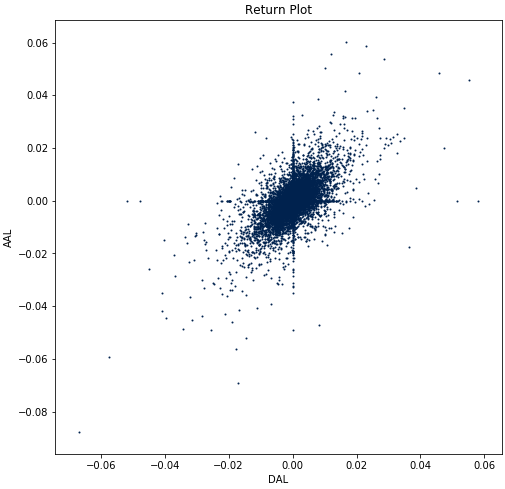
\includegraphics[width=.95\linewidth]{../Figures/return_plot_out.png}
    \caption{Returns with Outliers}
  \end{subfigure}%
  \begin{subfigure}{.5\textwidth}
    \centering
    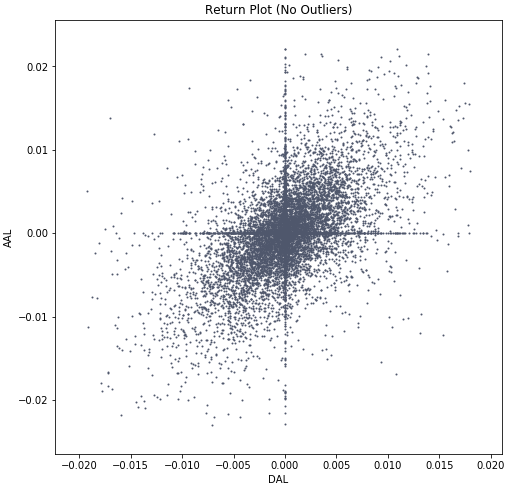
\includegraphics[width=.95\linewidth]{../Figures/return_plot_no_out.png}
    \caption{Returns with Outliers Removed}
  \end{subfigure}
  \caption{Impact of Outliers on Data}
\end{figure}
In order for the models to be able to learn the usual relationship between the securities, I used
the middle 99\% of data \textit{for training only}. The models were still evaluated on train and
test data that included outliers. The outlier removal was solely done to improve the fit of the
linear models.


\subsection{Returns and Markouts}
\subsubsection{Returns}
Asset returns represent 
a scaled first difference in the data, so they eliminate the serial component in the 
time series data along with its associated complications. The actual return 
as mentioned above can be defined as follows:
$$a_t = \frac{P_t - P_{t-1}}{P_{t-1}}$$
Normal approximations
have been used for asset returns on the monthly time scale, however, over short intervals this
assumption breaks down. The hourly returns used in this study are abundant close to 0 and 
extreme returns occur with greater frequency than under normality assumptions.
Despite this fact, OLS is a \textit{BLUE} estimator, so we can still confidently estimate 
a line despite the distribution not being normal. 
\subsubsection{Markouts}
Markouts are a way of computing hypothetical trade profits or losses. At every point along the
time series, we hypothetically enter a trade and hold for some predefined number of time 
periods, after which we exit the trade. Note that the entry can be a selling (short selling)
or buying trade, while the exit is simply the opposite side of the entry transaction. To 
specify this more rigorously, we can write:
$$M_{t,k} = \begin{cases} 
P_{t+k} - P_t \text { if Buy}\\
P_t - P_{t+k} \text { if Sell}
\end{cases}$$
This is the markout at time $t$, held for $k$ periods. Notice that $M^B_{t,k} = -M^S_{t,k}$,
meaning that the profit or loss of a buying and selling trade at a given point in time are 
exact opposites (since the asset can only move one direction). A good trading signal is one
that is able to separate positive from negative markouts. 

\section{Pairwise Mean Reversion}
As mentioned in the introduction, airline companies are exposed to similar pools of
risk. Oil companies are also exposed to similar pools of risk. Airline and oil companies
are both exposed to the price risk of oil itself, so it would stand to reason that the
stock prices of companies in this sector would move together. This assumption underpins
the pairwise mean reversion models presented in this section.
\subsection{Pairwise Correlations}
To get an idea of the relationships present among the companies in the data set, a pairwise
correlation analysis was conducted on the hourly returns of each of the securities.
\begin{figure}[h!]
  \centering
    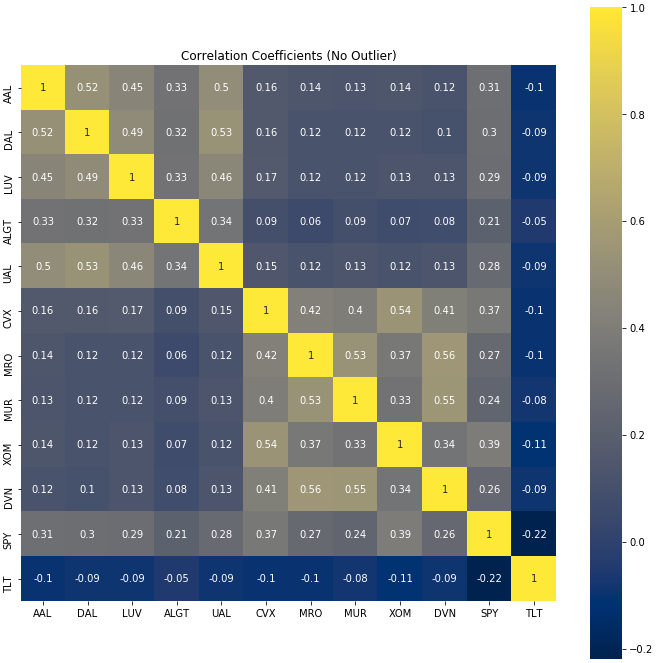
\includegraphics[width=.6\linewidth]{../Figures/pair_corr_no_out.png}
    \caption{Pairwise Correlation - Outliers Removed}
\end{figure}
We can see from Figure 1 above and section 6.3 in the appendix that the outliers in the 
data set had a noticeable positive impact on the correlations between the securities,
so for training purposes, it was appropriate to remove them. There are clear sections
of correlatedness in Figure 2 above. We can see that the 5 airline companies are together
correlated, while the same can be said for the 5 oil companies in the data set. There is also
some positive correlation between the companies in the data set and the S\&P 500 as well as some
negative correlation with price of bonds.

\subsection{Pairwise OLS}
With this understanding of the correlations between the data as well as the fact that
the outlier free return data exhibits ellipsoidal linear relationships, it became clear
that OLS would be a good model for this data. OLS was able to fit lines to the data well,
however, because the data fail to satisfy some assumptions of OLS, inference on the 
OLS parameters was not possible. The coefficients of the pairwise OLS model can be found
in Figure 3(a).
\begin{figure}[h!]
  \centering
  \begin{subfigure}{.5\textwidth}
    \centering
    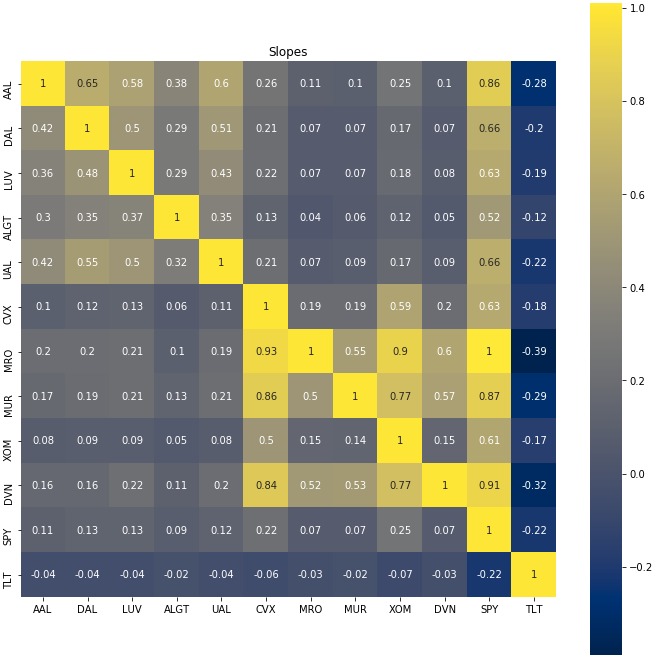
\includegraphics[width=.95\linewidth]{../Figures/pair_reg_slope.png}
    \caption{Model Slope Coefficient}
  \end{subfigure}%
  \begin{subfigure}{.5\textwidth}
    \centering
    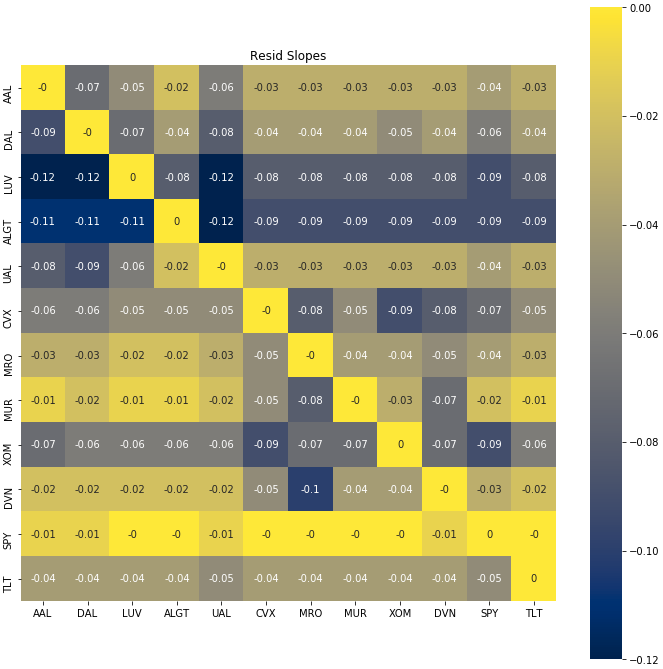
\includegraphics[width=.95\linewidth]{../Figures/pair_resid_reg_slope.png}
    \caption{Residual Slope Coefficient}
  \end{subfigure}
  \caption{Pairwise OLS, Y Axis Response}
\end{figure}
We see that the the strength of the slope coefficients lines up well with the strength of the
pairwise correlation between the assets. The intercept terms for these models were essentially
all zero. This can be seen in section 6.5. As defined in section 1.1, the idea behind
a statistical mean reverting trading strategy is to make bets on convergence to a forecasted
mean return. In this case, the mean return is the return for company $Y$ predicted 
at time $t$ using company $X$'s return under the pairwise model. The model makes money 
if when there is a negative residual on the model, the future return is positive, and
likewise if there is a positive residual on the model, the future return is negative.
In order to test if this is possible, we can run a regression on model residuals to 
future returns. The results of this can be found in Figure 3(b).
\begin{figure}[h!]
  \centering
  \begin{subfigure}{.5\textwidth}
    \centering
    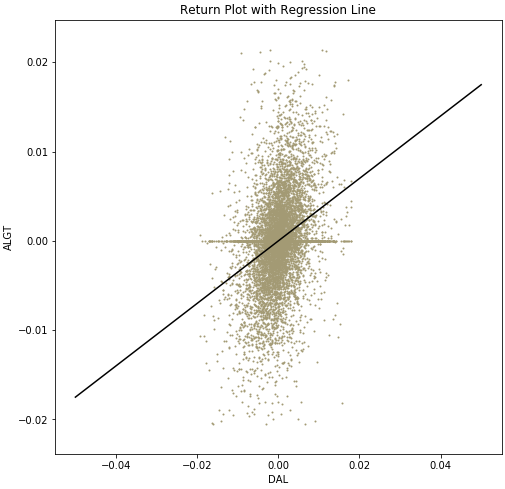
\includegraphics[width=.95\linewidth]{../Figures/return_plot_wReg.png}
    \caption{OLS Fit on No Outlier Data}
  \end{subfigure}%
  \begin{subfigure}{.5\textwidth}
    \centering
    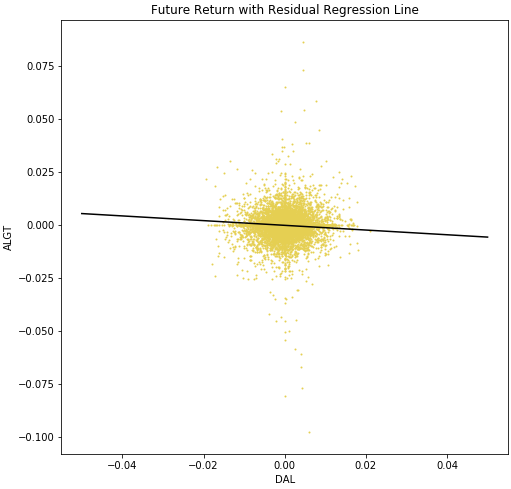
\includegraphics[width=.95\linewidth]{../Figures/return_plot_wResidReg.png}
    \caption{Future Returns Regressed on Model residuals}
  \end{subfigure}
  \caption{Return Plots with Regression}
\end{figure}
We see that there are some pairs with negative coefficients, which indicates that 
there is a relationship present. Such an example is shown in Figure 4. On the left
we see the regression model over the training set, while on the right we see the 
future returns regression model. There is a distinct downward slope in the model, but 
again, because the data fails OLS assumptions, we cannot tell whether the coefficient
is significant. Analysis on whether this strategy is good or not is presented in the
following section.

\subsection{Profit and Loss Analysis}
In order to assess whether the trading strategy is profitable, I introduce the notion
of a Profit and Loss (Pnl) Curve derived from cumulative markouts of trades taken
according to some signal parameter. Recalling the definition of markouts from section
1.3.2, as well as the fact that our trading signal for this model is the size 
of the model residual, we can generate a PnL curve on the \textit{test} set.
We define this as follows:
$$\mathrm{PnL}(\lambda)_k^B = \sum_{t=1}^n \Phi_B(\lambda, r_t) M_{t,k}^B
\quad
\Phi_B(\lambda, r_t) = \begin{cases}
  1 \text { if } r_t < \lambda\\
  0 \text { if } r_t > \lambda  
\end{cases}$$
$$\mathrm{PnL}(\lambda)_k^S = \sum_{t=1}^n \Phi_S(\lambda, r_t) M_{t,k}^S
\quad
\Phi_S(\lambda, r_t) = \begin{cases}
  1 \text { if } r_t > \lambda\\
  0 \text { if } r_t < \lambda  
\end{cases}$$
Where $\Phi$ is an indicator function to determine how the residual relates to the
signal threshold $\lambda$. The curves for buying and selling PnL can be seen below
in Figure 5. I chose a signal threshold of $\lambda=0$ by observing the peaks
of these curves on \textit{train} data, and they are applied here on \textit{test}
data.
\begin{figure}[h!]
  \centering
  \begin{subfigure}{.5\textwidth}
    \centering
    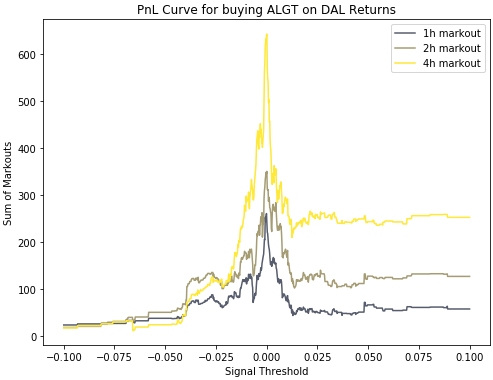
\includegraphics[width=.95\linewidth]{../Figures/pair_Pnl_Curve_buy_ALGT_on_DAL.png}
    \caption{Buy Side PnL}
  \end{subfigure}%
  \begin{subfigure}{.5\textwidth}
    \centering
    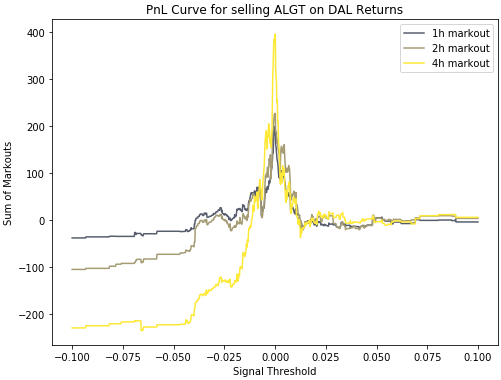
\includegraphics[width=.95\linewidth]{../Figures/pair_Pnl_Curve_sell_ALGT_on_DAL.png}
    \caption{Sell Side PnL}
  \end{subfigure}
  \caption{Pairwise Pnl Curves - ALGT}
\end{figure}
The shape of the curve follows from intuition, at the left end of the buying curve, there
are no data points with a sufficiently negative residual for us to buy, so the PnL is 0,
while at the right end, we are making every possible trade. Because the market went
up for a large part of 2020 and 2021 (except for the March 2020 crash), it makes sense
that we come out positive if we buy all the time. 
We can see that there are noticeable peaks at 0 for both buying and selling PnL, which
further justifies the choice of 0 as a threshold parameter. The PnL for a
0 threshold is reported in Figure 6 below.
\begin{figure}[h!]
  \centering
  \begin{subfigure}{.5\textwidth}
    \centering
    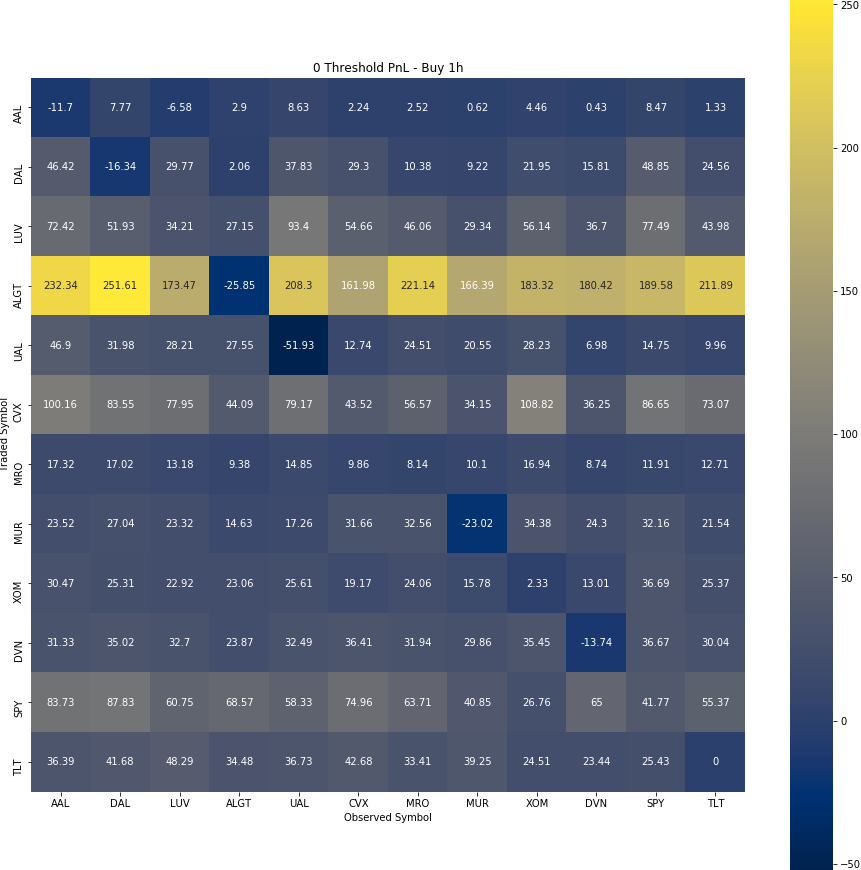
\includegraphics[width=.95\linewidth]{../Figures/pair_buy_pnl_1h.png}
    \caption{Buy Side PnL}
  \end{subfigure}%
  \begin{subfigure}{.5\textwidth}
    \centering
    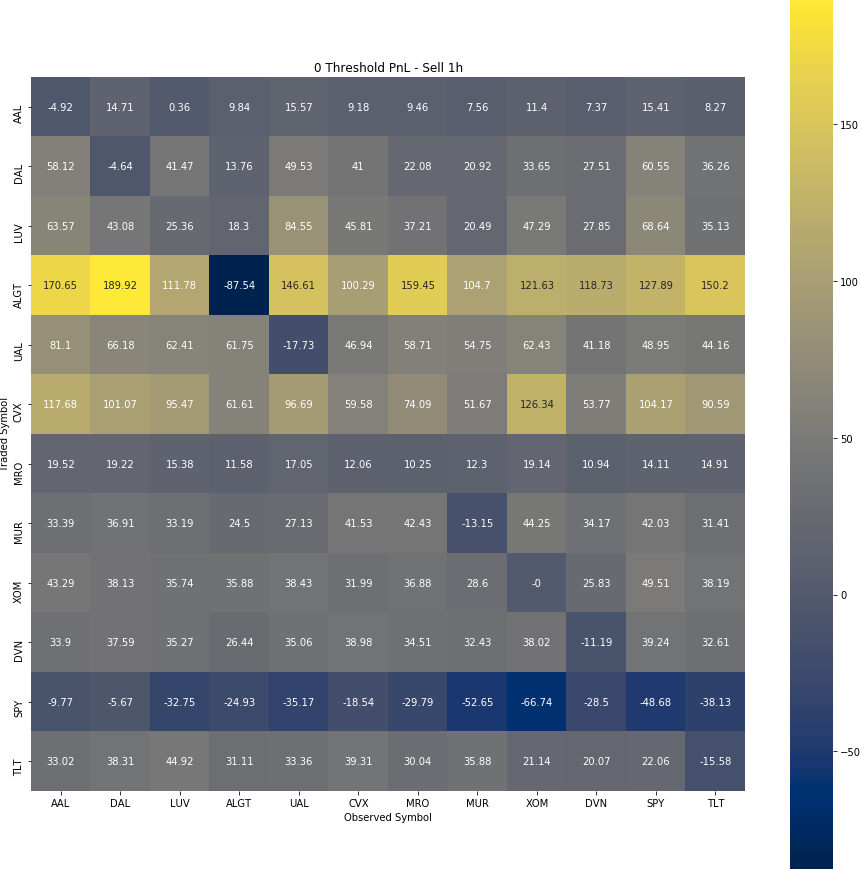
\includegraphics[width=.95\linewidth]{../Figures/pair_sell_pnl_1h.png}
    \caption{Sell Side PnL}
  \end{subfigure}
  \caption{1-Hour Markouts}
\end{figure}
Surprisingly, most of the pairs are profitable, with Allegiant Airlines standing out 
as one of the most profitable companies to trade, likely due to its volatility, which
can be seen in Figure 4(a). The ellipse is very steep, meaning that for
returns in Delta Airlines stock, Allegiant stock is quite volatile.

\section{Basket Mean Reversion using Principal Components}
Having seen the success of the pairwise analyses and the positive markouts for 
a $\lambda=0$ signal, one might wonder what improvements could be had by including
more predictors in the regression models. However, the returns of the stocks in the 
data set are correlated (Figure 2) and in some cases would be prohibitively multicollinear under
an OLS model. In order to solve this problem, we can transform the returns into
orthogonal principal components and regress on the transformed data. 

\subsection{Orthogonal Transformation}
In order to prevent data leakage, the target variable was held out of the data set before 
a transformation was applied. I examined many possible subsets of data over which 
diagonalization and regression was performed (airlines on airlines, oil on oil, all on all).
The best results from an RMSE perspective mandated that all of the stocks (except for the 
target) be included in the principal component transformation. This can be seen in section
6.1 and will be discussed further in section 3.2. The following analysis applies
to the principal components extracted over all the data. 

\begin{figure}[h!]
  \centering
  \begin{subfigure}{.5\textwidth}
    \centering
    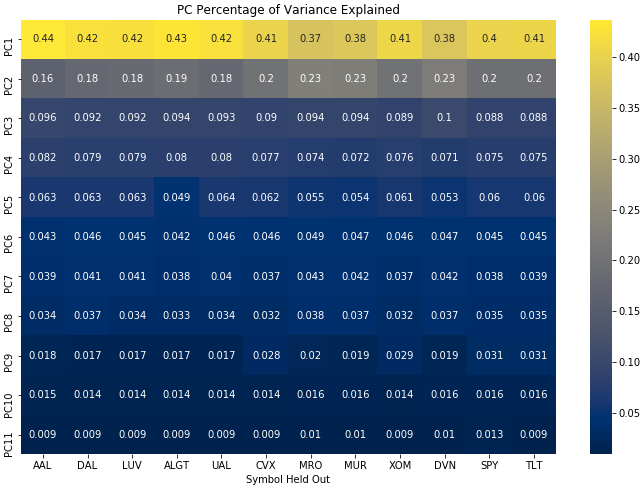
\includegraphics[width=.95\linewidth]{../Figures/PCA_pve.png}
    \caption{PCA Percentage of Variance Explained}
  \end{subfigure}%
  \begin{subfigure}{.5\textwidth}
    \centering
    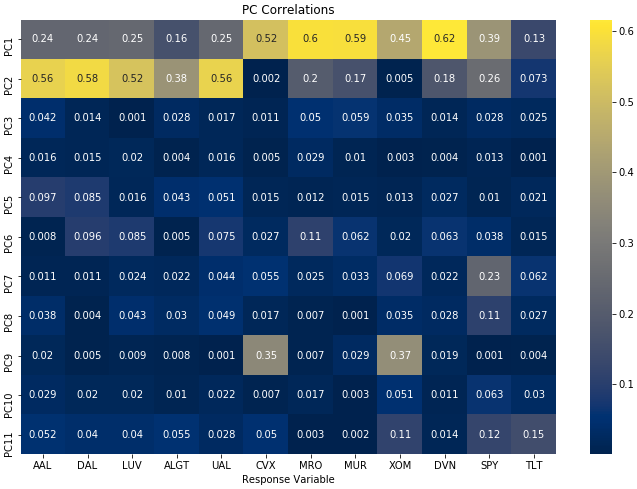
\includegraphics[width=.95\linewidth]{../Figures/PCA_corr_resp.png}
    \caption{Principal Component Correlation with Response}
  \end{subfigure}
  \caption{PCA Metrics}
\end{figure}
In Figure 7, we can see the results of the principal component decomposition. As expected,
due to the correlations in the data, we see that the first principal component explains
a significant proportion of the variance. For smaller subsets of data, say airlines,
the first principal component explained upwards of 60\% of the variance. The 
interesting observation however, is that the returns of the held out security do
not always have the highest correlation with the first principal component. For 
example, Chevron (CVX) and Exxon Mobil (XOM) seem to correlate with the 9th principal
component. This is especially interesting because from a business standpoint, CVX
and XOM are very similar.
\begin{figure}[h!]
  \centering
    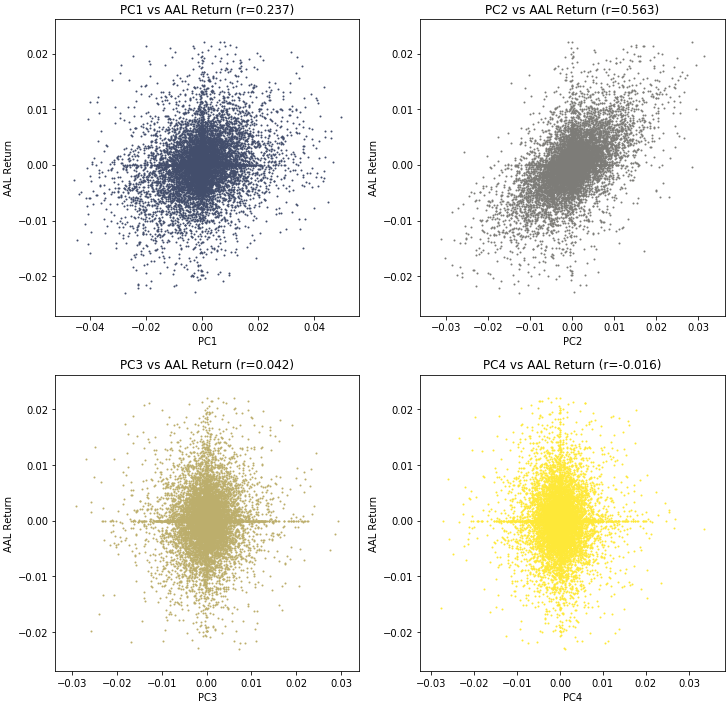
\includegraphics[width=.6\linewidth]{../Figures/PCA_plot.png}
    \caption{Decomposition Plot}
\end{figure}
In Figure 8 above, we can see the plot of American Airlines returns against the 
first 4 principal components of the other 11 stocks. We can also see there that
there appears to be a stronger relationship between AAL and PC2 than AAL and PC1.

\subsection{Basket OLS}
After fitting the principal componenst on \textit{train} data, and OLS model
was run with the held out symbol as response and the principal components as 
predictors. The coefficients of the principal components can be seen below in
Figure 9. We can also see that the intercept is not meaningfully different from 0.
\begin{figure}[h!]
  \centering
  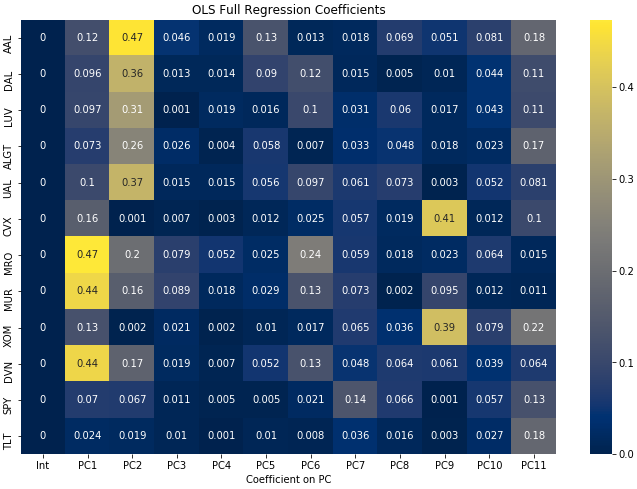
\includegraphics[width=.6\linewidth]{../Figures/Full_PCReg_coef.png}
  \caption{Full PC OLS Regression}
\end{figure}
An important thing to note is that this plot above, as well as the correlation plot
found in Figure 7 display absolute values of coefficients and correlations. Because
principal component analysis yields unique vectors, but not unique directions,
we can flip the signs of the values for easier visual analysis.
\subsubsection{Basket Lasso for Feature Selection}
As mentioned in the start of section 3.1, I examined several subsets of data and 
settled on the full principal component set as the best set of predictors for the model.
The model can be thought of as follows:
$$\hat x_{target} = f(T(\mathbf{X}_{-target}))
\quad
\mathbf{X} = \begin{bmatrix}x_{target}, \mathbf{X}_{-target}\end{bmatrix}
$$
where $T$ is the orthogonal transformation applied to the predictors and
$f$ is the function learned by OLS. Section 6.1
outlines several choices of $\mathbf{X}$ and their corresponding RMSE. I also applied
a lasso regression to the data with a cross validated tuning parameter for 
the impact of the L1 penalty, however, I found that the optimal loss penalty 
was very small and that the RMSE of the original OLS model was better in 
nearly every case. With this understanding, we can see that the best set
of features is the full set, and that the best model to use is in fact OLS.

\subsection{Profit and Loss Analysis}
The application of the PnL analysis in this scenario is the same as in section
2.3, and the formulas remain the same. However there is the caveat that now:
$$r_t = a_t - f(T(\mathbf{x}_{-target,t}))$$
We are using a transformed set of all the predictors to forecast the expected return
for an asset. It is important to note that the PCA fit and OLS fit were 
carried out on \textit{train} data, and that the same parameters were carried over 
to evaluate the \textit{test} data and produce the plots that are seen below.
\begin{figure}[h!]
  \centering
  \begin{subfigure}{.5\textwidth}
    \centering
    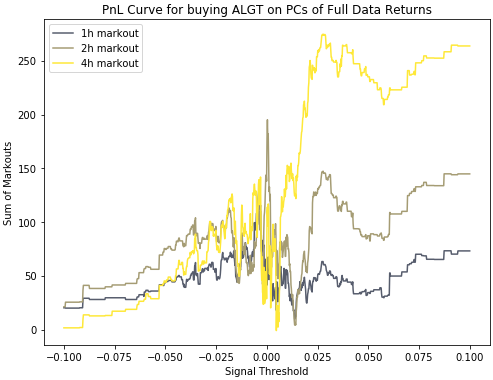
\includegraphics[width=.95\linewidth]{../Figures/basket_Pnl_Curve_buy_ALGT.png}
    \caption{Buy Side PnL}
  \end{subfigure}%
  \begin{subfigure}{.5\textwidth}
    \centering
    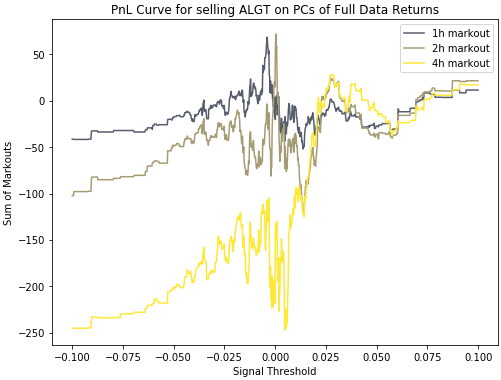
\includegraphics[width=.95\linewidth]{../Figures/basket_Pnl_Curve_sell_ALGT.png}
    \caption{Sell Side PnL}
  \end{subfigure}
  \caption{Basket Pnl Curves - ALGT}
\end{figure}
We can see in Figure 10 the PnL curves for Allegiant Airlines using all of the 
principal component predictors. They are substantially more noisy when compared to the 
plots in Figure 5, especially as the markout horizon grows longer. We can see
the results for a 0 threshold PnL for all of the securities in Figure 11 below.
\begin{figure}[h!]
  \centering
  \begin{subfigure}{.5\textwidth}
    \centering
    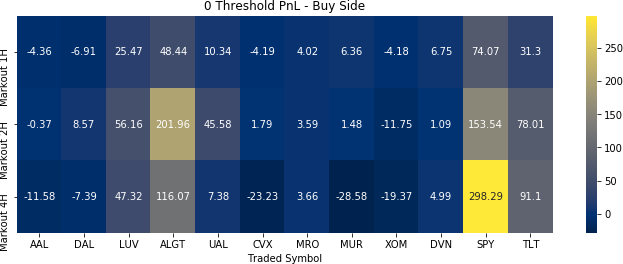
\includegraphics[width=.95\linewidth]{../Figures/basket_buy_pnl.png}
    \caption{Buy Side PnL}
  \end{subfigure}%
  \begin{subfigure}{.5\textwidth}
    \centering
    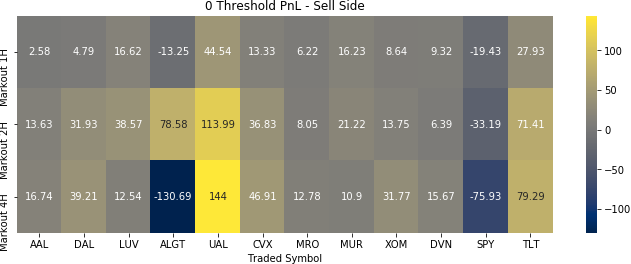
\includegraphics[width=.95\linewidth]{../Figures/basket_sell_pnl.png}
    \caption{Sell Side PnL}
  \end{subfigure}
  \caption{Basket Model PnL}
\end{figure}
It is clear that there is still some activity at $\lambda = 0$ occuring in the data,
however it is a lot more noisy. The threshold of 0 was maintained for ease of comparison
to the other model, however it is not necessarily the case that $\lambda=0$ is an optimal
threshold for this model, since it has different characteristics. Further discussion 
can be found below.

\section{Discussion}
The unexpected element of this analysis is the fact that the basket model with more
data and more meticulous preprocessing of that data happens to perform worse
than the comparatively simple pairwise model. There are several possible explanations
for this and I will touch on a handful below.
\subsection{The Compounding Outlier Problem}
The breakdown of the full principal component model could
be attributed to what I would call the "compounding outlier problem". The test set contains
data from 2020 and 2021, and 2020 was a very volatile year with several extreme price 
moves for airline and oil companies. These were driven primarily by the shutdown 
of travel due to the pandemic and the brief period in April 2020 when the price of 
oil was negative. However, even apart from the pandemic setting, the models in this
study were fitted on outlier trimmed data. When evaluated on a pairwise basis,
there is some chance of encountering an outlier at any given point in time in the 
predictor series. However, when using $k$ predictor series in the model, there
are $2^k$ possible scenarios in which outliers might play a role at any time $t$. 
These outliers are thus more likely to be present in the larger model and can
throw off the predictions substantially more often. 

\subsection{Poor Feature Selection}
Another possible explanation for the lackluster performance of the basket model could
be attributed to poor feature selection. Based on the correlation matrix found 
in Figure 2, it is hard to claim that each company's stock depends on all of the 
other companies. The TLT ETF is a great example - it doesn't seem to relate well to 
any of companies. Yet, after a principal component analysis, the left over
principal components with rather poor correlation to the target are not dropped 
by Lasso Regression. This could be due to the distribution of the data. There is 
and abundance of hourly returns centered around or exactly equal to 0, and the outliers
that were not removed (but rightfully deemed outliers) drive the fit to such an 
extent that Lasso Regression neglects to shrink their coefficients.

\subsection{Assumption Breakdown}
It is perhaps always the case that assumption breakdown is at least in part responsible 
for poor model performance. In this context, I don't refer to statistical assumptions,
though the outliers may have had an impact as mentioned in section 4.1. Instead
I refer to the stationarity assumptions made about the correlations between
asset classes. This style of statistical mean reversion trading strategies relies
on a continued statistical relationship between assets, which may cease to exist at 
any point in time. 2020 was a great example of this because long standing correlations 
between assets (eg. inverse correlation of S\&P 500 and Gold) broke down. It could 
very well be the case that it is not reasonable to make convergence bets in the period
defined by the test set.

\section{Conclusion}
This paper highlights two statistical mean reversion trading strategies and evaluates
them on their peak signal profit or loss. The simpler pairwise trading strategy 
outperformed the basket strategy that utilized a larger set of features and principal
component analysis to preprocess and select these features. On the surface, this is a
counterintuitive result because one might believe that more data allows for better 
models. However, the deterioration of the basket strategy indicates the potentially
problematic effects of higher dimensional data. In order to achieve comparable quality
and interpretability in results, one needs exponentially cleaner data that 
is analyzed in a substantially more rigourous fashion. 

This type of mean reverting signal shows promise, and the next steps for this 
analysis will likely be an implementation of this strategy in a backtest or 
simulation context. It is important to note that any positive results in this 
paper do not guarantee positive results while trading live, so readers should
exercise caution if they decide to implement any of the ideas discussed in this paper.

\newpage
\section{Appendix}

\subsection{RMSE for PC Regression Models}
\begin{table}[!htb]
    \begin{minipage}{.5\linewidth}
      \caption{Airline PC Regression RMSE}
      \centering
      \begin{tabular}{ c|c|c|c }
        \textbf{Ticker} & \textbf{PC1} & \textbf{Full} & \textbf{Lasso} \\
        \hline
        AAL	& 0.003519 & 0.003487 & 0.003487\\
        DAL	& 0.002762 & 0.002725 & 0.002725\\
        LUV	& 0.002839 & 0.002819 & 0.002819\\
        ALGT & 0.003561 & 0.003554 & 0.003554\\
        UAL	& 0.002931 & 0.002902 & 0.002902\\
        \end{tabular}
    \end{minipage}%
    \begin{minipage}{.5\linewidth}
      \centering
        \caption{Oil PC Regression RMSE}
        \begin{tabular}{ c|c|c|c  }
            \textbf{Ticker} & \textbf{PC1} & \textbf{Full} & \textbf{Lasso} \\
            \hline
            CVX	& 0.002338	& 0.002136	& 0.002136\\
            MRO	& 0.004708	& 0.004647	& 0.004647\\
            MUR	& 0.004573	& 0.004536	& 0.004536\\
            XOM	& 0.002240	& 0.002047	& 0.002047\\
            DVN	& 0.004302	& 0.004281	& 0.004284\\
        \end{tabular}
    \end{minipage} 
\end{table}

\begin{table}[!htb]
    \begin{minipage}{.5\linewidth}
      \caption{Airline and Oil PC Regression RMSE}
      \centering
      \begin{tabular}{ c|c|c|c }
        \textbf{Ticker} & \textbf{PC1} & \textbf{Full} & \textbf{Lasso} \\
        \hline
        AAL	& 0.004306	& 0.003475	& 0.003478\\
        DAL	& 0.003450	& 0.002721	& 0.002722\\
        LUV	& 0.003363	& 0.002809	& 0.002809\\
        ALGT & 0.003865	& 0.003552	& 0.003553\\
        UAL	& 0.003602	& 0.002896	& 0.002896\\
        CVX	& 0.002320	& 0.002124	& 0.002125\\
        MRO	& 0.004851	& 0.004640	& 0.004641\\
        MUR	& 0.004661	& 0.004530	& 0.004530\\
        XOM	& 0.002231	& 0.002044	& 0.002044\\
        DVN	& 0.004414	& 0.004275	& 0.004278\\
        \end{tabular}
    \end{minipage}%
    \begin{minipage}{.5\linewidth}
      \centering
        \caption{Full PC Regression RMSE}
        \begin{tabular}{ c|c|c|c  }
            \textbf{Ticker} & \textbf{PC1} & \textbf{Full} & \textbf{Lasso} \\
            \hline
            AAL	& 0.004301	& 0.003458	& 0.003458\\
            DAL	& 0.003446	& 0.002713	& 0.002713\\
            LUV	& 0.003359	& 0.002801	& 0.002801\\
            ALGT & 0.003863	& 0.003543	& 0.003545\\
            UAL	& 0.003598	& 0.002891	& 0.002891\\
            CVX	& 0.002316	& 0.002104	& 0.002105\\
            MRO	& 0.004854	& 0.004634	& 0.004635\\
            MUR	& 0.004666	& 0.004530	& 0.004531\\
            XOM	& 0.002227	& 0.001996	& 0.001996\\
            DVN	& 0.004418	& 0.004271	& 0.004275\\
            SPY	& 0.001469	& 0.001329	& 0.001330\\
            TLT	& 0.001574	& 0.001546	& 0.001546\\
        \end{tabular}
    \end{minipage} 
\end{table}

\newpage
\subsection{Return Plots}
\begin{figure}[h!]
  \centering
  \begin{subfigure}{.5\textwidth}
    \centering
    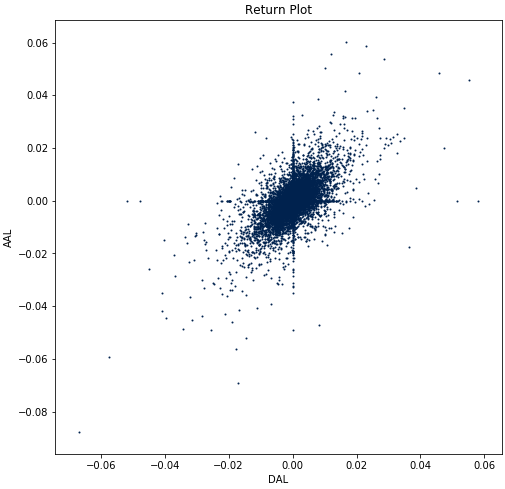
\includegraphics[width=.95\linewidth]{../Figures/return_plot_out.png}
    \caption{Returns with Outliers}
  \end{subfigure}%
  \begin{subfigure}{.5\textwidth}
    \centering
    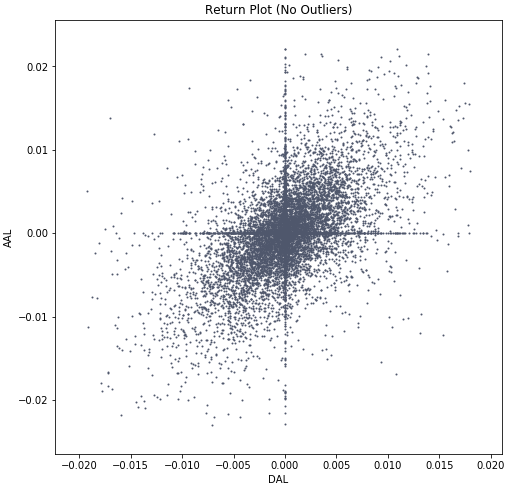
\includegraphics[width=.95\linewidth]{../Figures/return_plot_no_out.png}
    \caption{Returns with Outliers Removed}
  \end{subfigure}
  \caption{Impact of Outliers on Data}
\end{figure}

\begin{figure}[h!]
  \centering
  \begin{subfigure}{.5\textwidth}
    \centering
    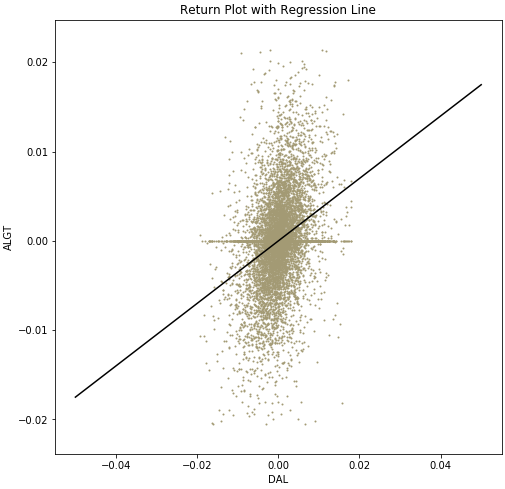
\includegraphics[width=.95\linewidth]{../Figures/return_plot_wReg.png}
    \caption{OLS Fit on No Outlier Data}
  \end{subfigure}%
  \begin{subfigure}{.5\textwidth}
    \centering
    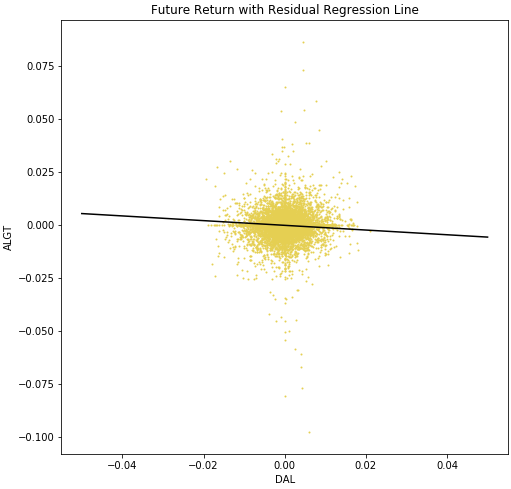
\includegraphics[width=.95\linewidth]{../Figures/return_plot_wResidReg.png}
    \caption{Future Returns Regressed on Model residuals}
  \end{subfigure}
  \caption{Return Plots with Regression}
\end{figure}

\newpage
\subsection{Correlations}
\begin{figure}[h!]
  \centering
    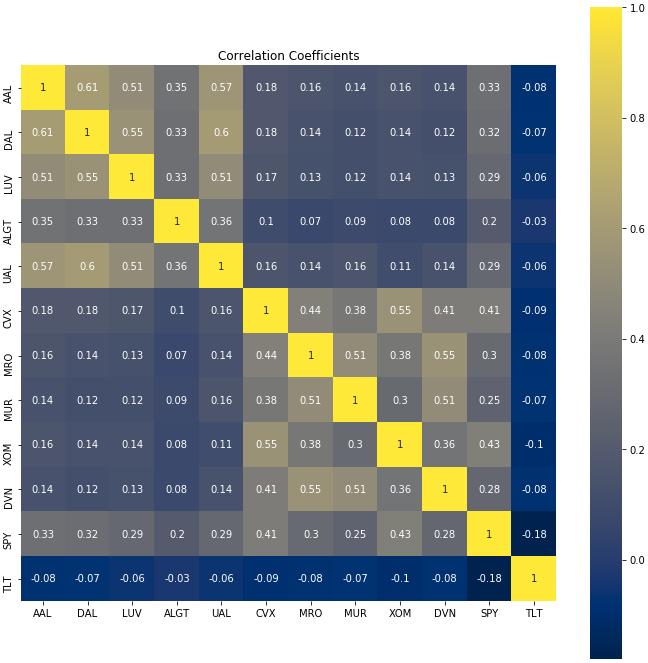
\includegraphics[width=.5\linewidth]{../Figures/pair_corr_out.png}
    \caption{Pairwise Correlation - Outliers Present}
\end{figure}
\begin{figure}[h!]
  \centering
    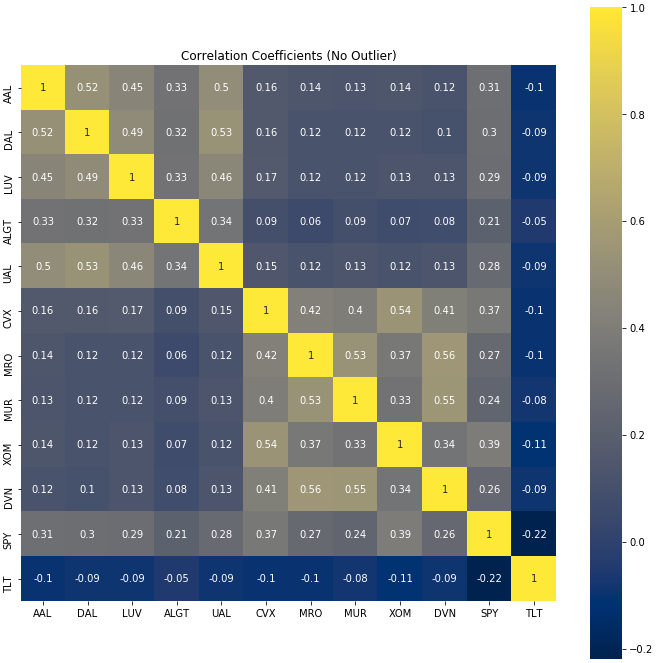
\includegraphics[width=.5\linewidth]{../Figures/pair_corr_no_out.png}
    \caption{Pairwise Correlation - Outliers Removed}
\end{figure}

\newpage
\subsection{Principal Component Analysis}
\begin{figure}[h!]
  \centering
    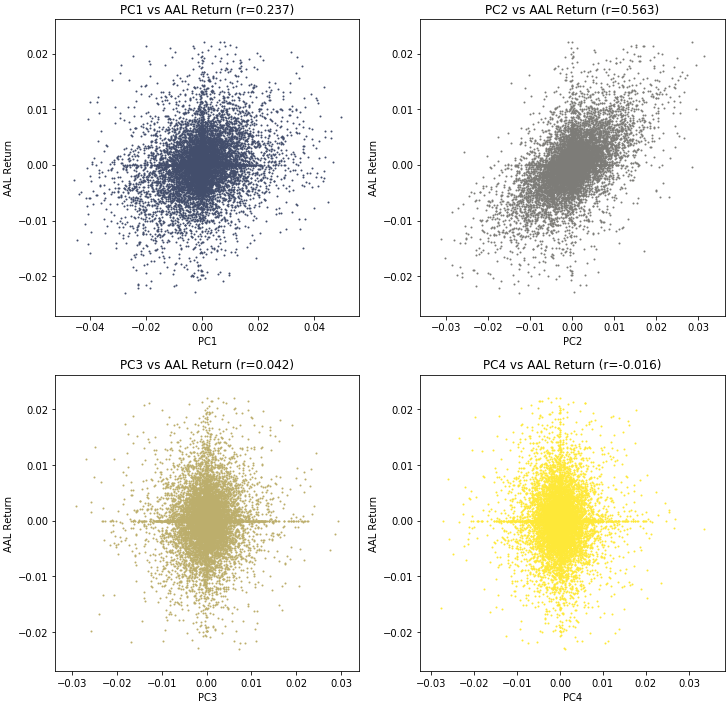
\includegraphics[width=.8\linewidth]{../Figures/PCA_plot.png}
    \caption{Decomposition Plot}
\end{figure}
\begin{figure}[h!]
  \centering
  \begin{subfigure}{.5\textwidth}
    \centering
    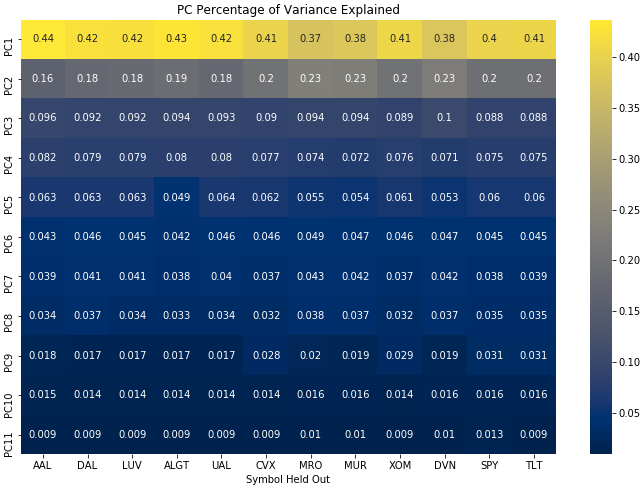
\includegraphics[width=.95\linewidth]{../Figures/PCA_pve.png}
    \caption{PCA Percentage of Variance Explained}
  \end{subfigure}%
  \begin{subfigure}{.5\textwidth}
    \centering
    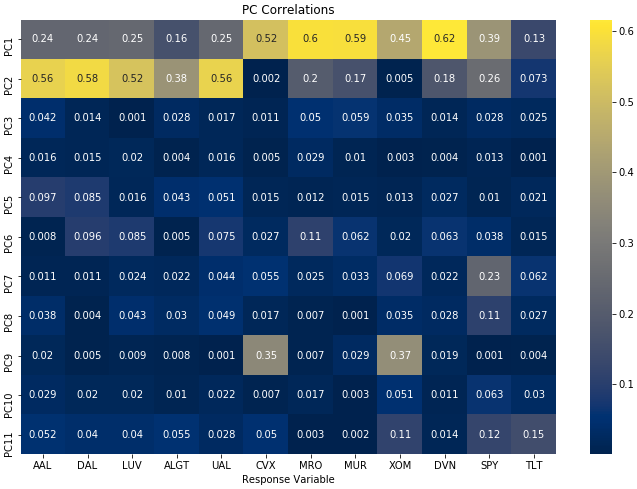
\includegraphics[width=.95\linewidth]{../Figures/PCA_corr_resp.png}
    \caption{Principal Component Correlation with Response}
  \end{subfigure}
  \caption{PCA Metrics}
\end{figure}

\newpage
\subsection{Regression Coefficients}

\subsubsection{Pairwise Regression}
\begin{figure}[h!]
  \centering
  \begin{subfigure}{.5\textwidth}
    \centering
    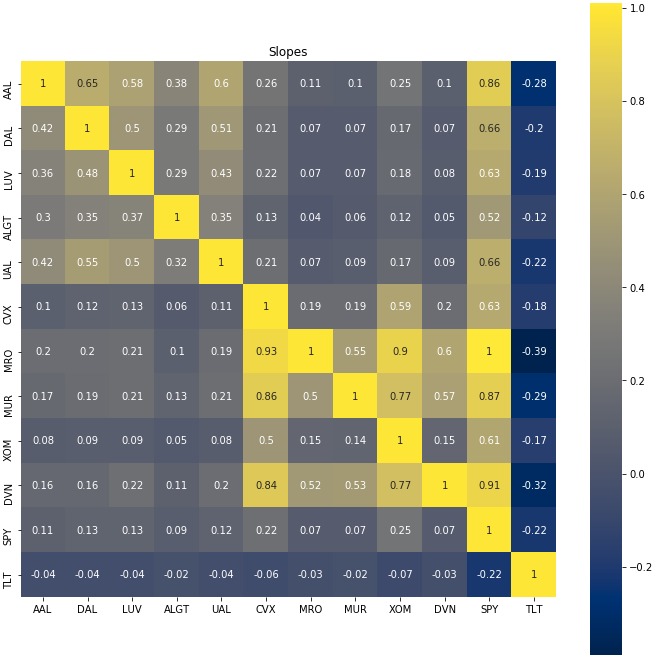
\includegraphics[width=.95\linewidth]{../Figures/pair_reg_slope.png}
    \caption{Slope Coefficient}
  \end{subfigure}%
  \begin{subfigure}{.5\textwidth}
    \centering
    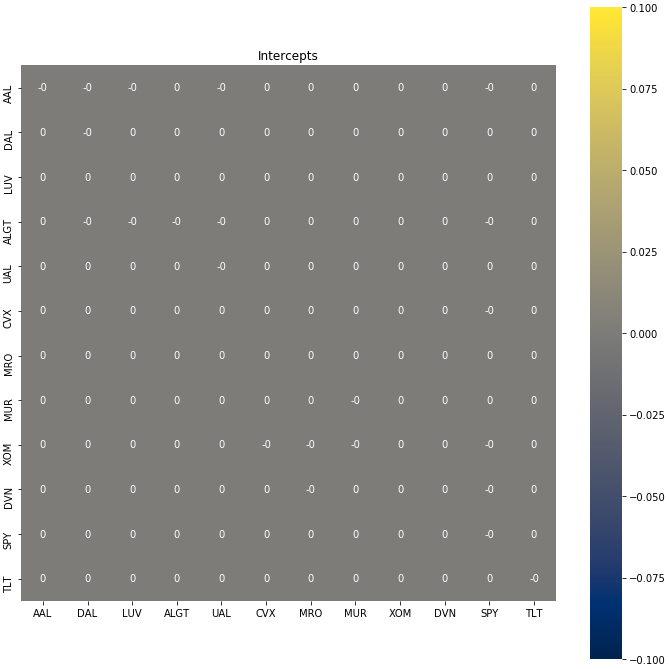
\includegraphics[width=.95\linewidth]{../Figures/pair_reg_intercept.png}
    \caption{Intercept}
  \end{subfigure}
  \caption{Pairwise Regression}
\end{figure}

\subsubsection{Pairwise Residual Regression}
\begin{figure}[h!]
  \centering
  \begin{subfigure}{.5\textwidth}
    \centering
    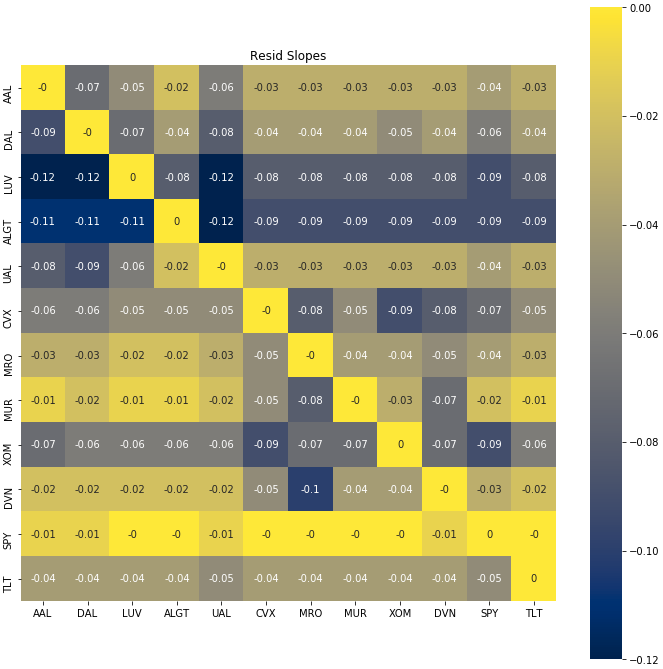
\includegraphics[width=.95\linewidth]{../Figures/pair_resid_reg_slope.png}
    \caption{Slope Coefficient}
  \end{subfigure}%
  \begin{subfigure}{.5\textwidth}
    \centering
    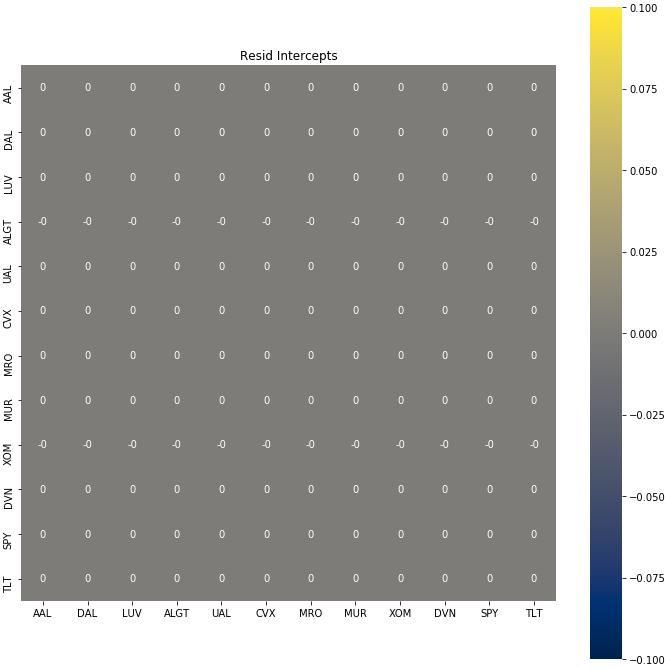
\includegraphics[width=.95\linewidth]{../Figures/pair_resid_reg_intercept.png}
    \caption{Intercept}
  \end{subfigure}
  \caption{Pairwise Residual Regression}
\end{figure}

\subsubsection{Principal Component Regression}
\begin{figure}[h!]
  \centering
    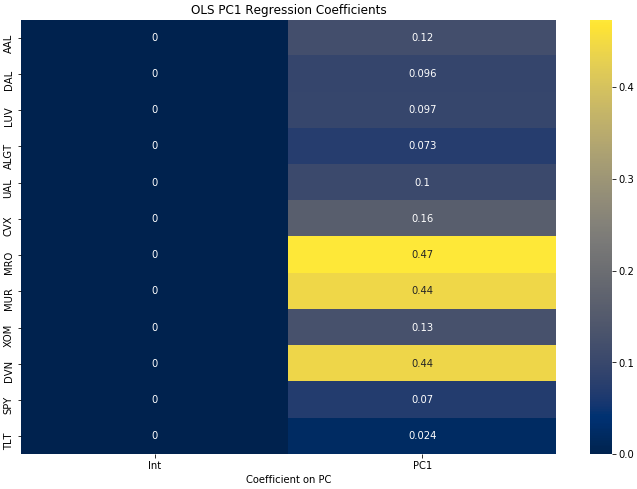
\includegraphics[width=.4\linewidth]{../Figures/PC1_PCReg_coef.png}
    \caption{PC1 OLS Regression}
\end{figure}
\begin{figure}[h!]
    \centering
    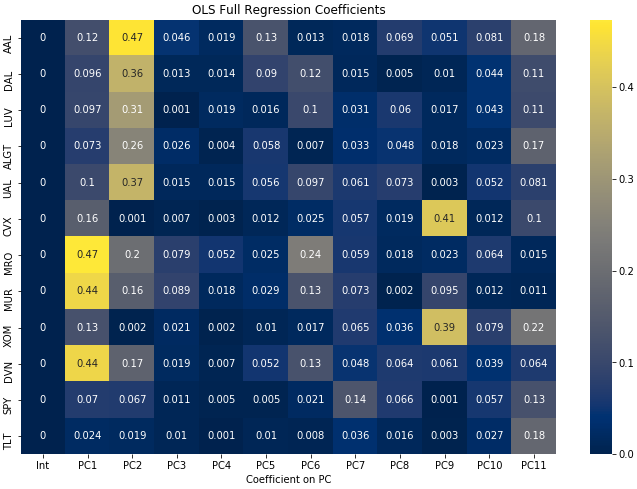
\includegraphics[width=.4\linewidth]{../Figures/Full_PCReg_coef.png}
    \caption{Full PC OLS Regression}
\end{figure}
\begin{figure}[h!]
    \centering
    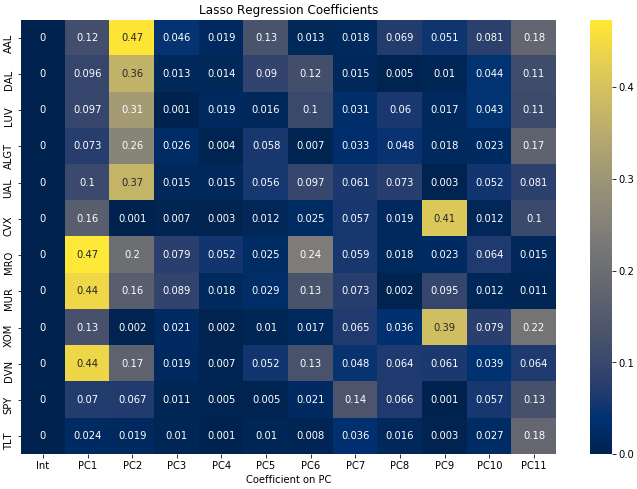
\includegraphics[width=.4\linewidth]{../Figures/Lasso_PCReg_coef.png}
    \caption{Lasso PC Regression}
\end{figure}

\newpage
\subsection{Profit and Loss Signal Curves}
\begin{figure}[h!]
  \centering
  \begin{subfigure}{.5\textwidth}
    \centering
    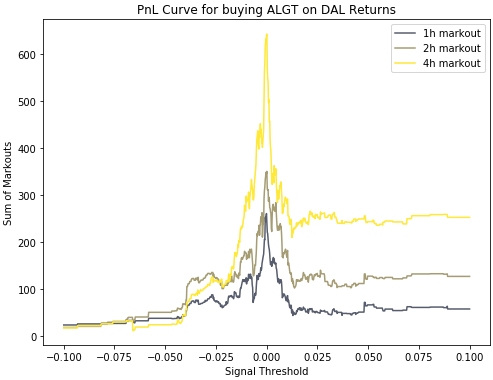
\includegraphics[width=.95\linewidth]{../Figures/pair_Pnl_Curve_buy_ALGT_on_DAL.png}
    \caption{Buy Side PnL}
  \end{subfigure}%
  \begin{subfigure}{.5\textwidth}
    \centering
    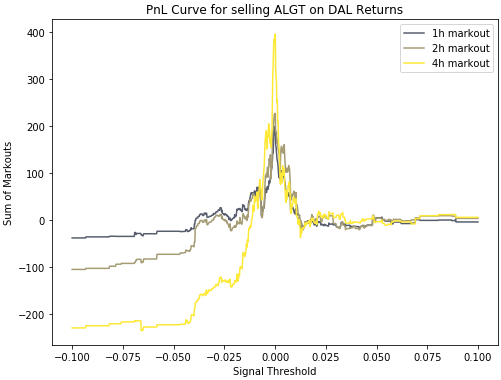
\includegraphics[width=.95\linewidth]{../Figures/pair_Pnl_Curve_sell_ALGT_on_DAL.png}
    \caption{Sell Side PnL}
  \end{subfigure}
  \caption{Pairwise Pnl Curves - ALGT}
\end{figure}

\begin{figure}[h!]
  \centering
  \begin{subfigure}{.5\textwidth}
    \centering
    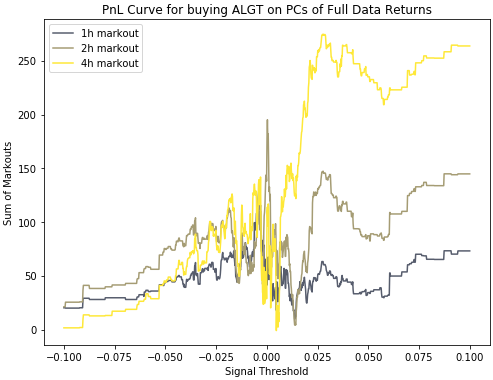
\includegraphics[width=.95\linewidth]{../Figures/basket_Pnl_Curve_buy_ALGT.png}
    \caption{Buy Side PnL}
  \end{subfigure}%
  \begin{subfigure}{.5\textwidth}
    \centering
    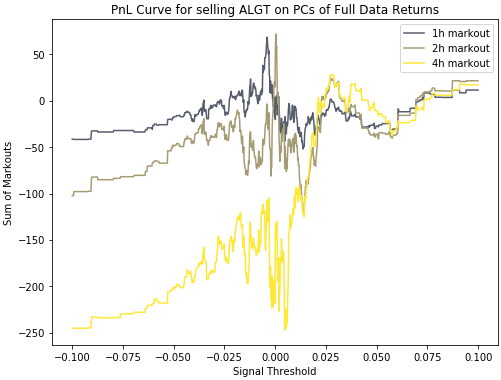
\includegraphics[width=.95\linewidth]{../Figures/basket_Pnl_Curve_sell_ALGT.png}
    \caption{Sell Side PnL}
  \end{subfigure}
  \caption{Basket Pnl Curves - ALGT}
\end{figure}

\newpage
\subsection{Profit and Loss over Markout Horizons}
\begin{figure}[h!]
  \centering
  \begin{subfigure}{.5\textwidth}
    \centering
    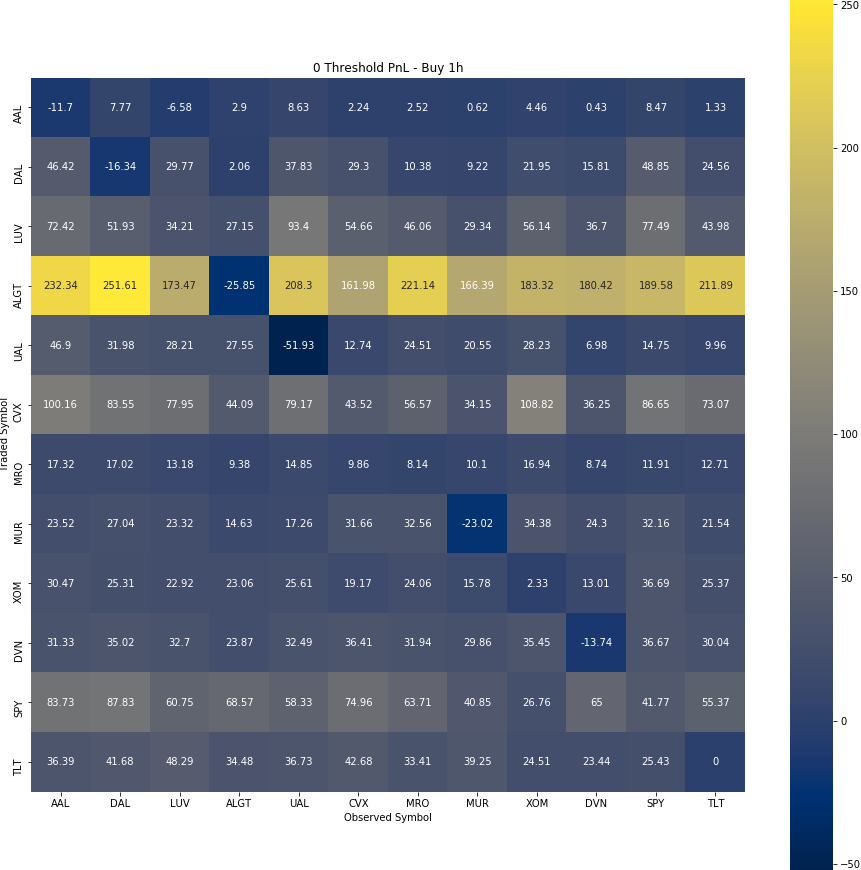
\includegraphics[width=.95\linewidth]{../Figures/pair_buy_pnl_1h.png}
    \caption{Buy Side PnL}
  \end{subfigure}%
  \begin{subfigure}{.5\textwidth}
    \centering
    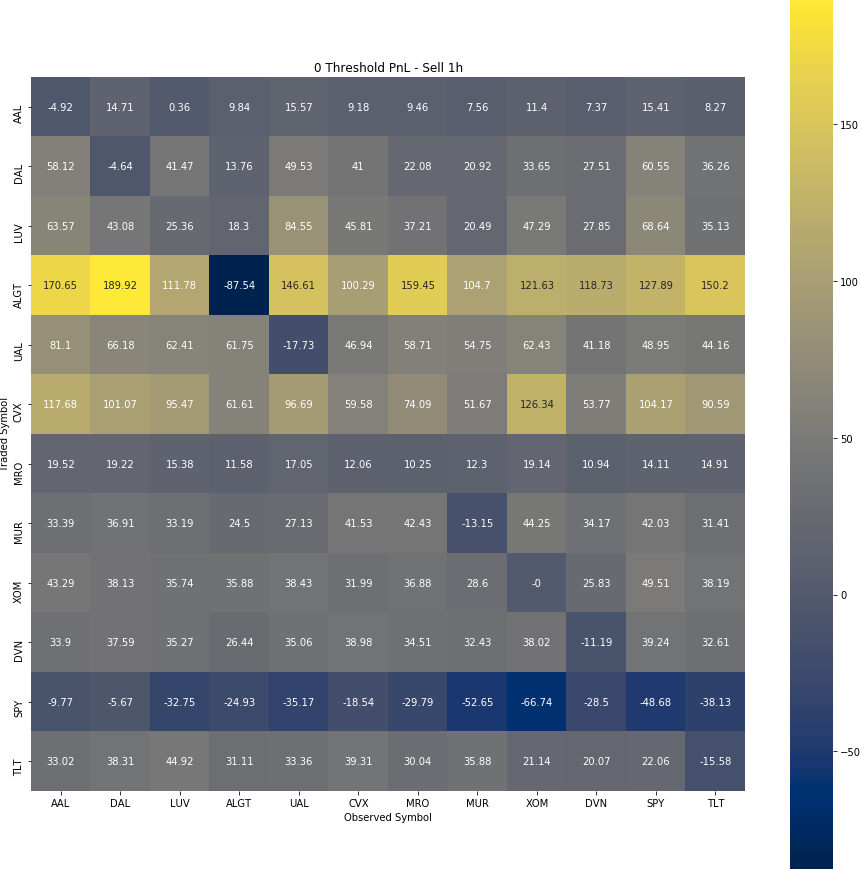
\includegraphics[width=.95\linewidth]{../Figures/pair_sell_pnl_1h.png}
    \caption{Sell Side PnL}
  \end{subfigure}
  \caption{1-Hour Markouts}
\end{figure}

\begin{figure}[h!]
  \centering
  \begin{subfigure}{.5\textwidth}
    \centering
    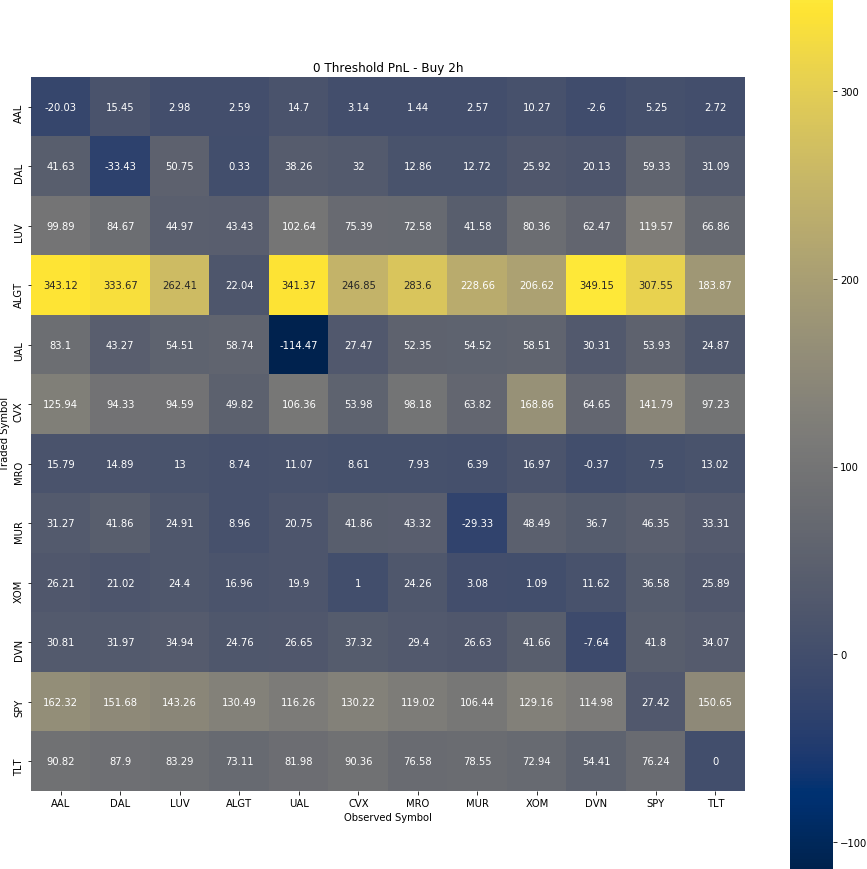
\includegraphics[width=.95\linewidth]{../Figures/pair_buy_pnl_2h.png}
    \caption{Buy Side PnL}
  \end{subfigure}%
  \begin{subfigure}{.5\textwidth}
    \centering
    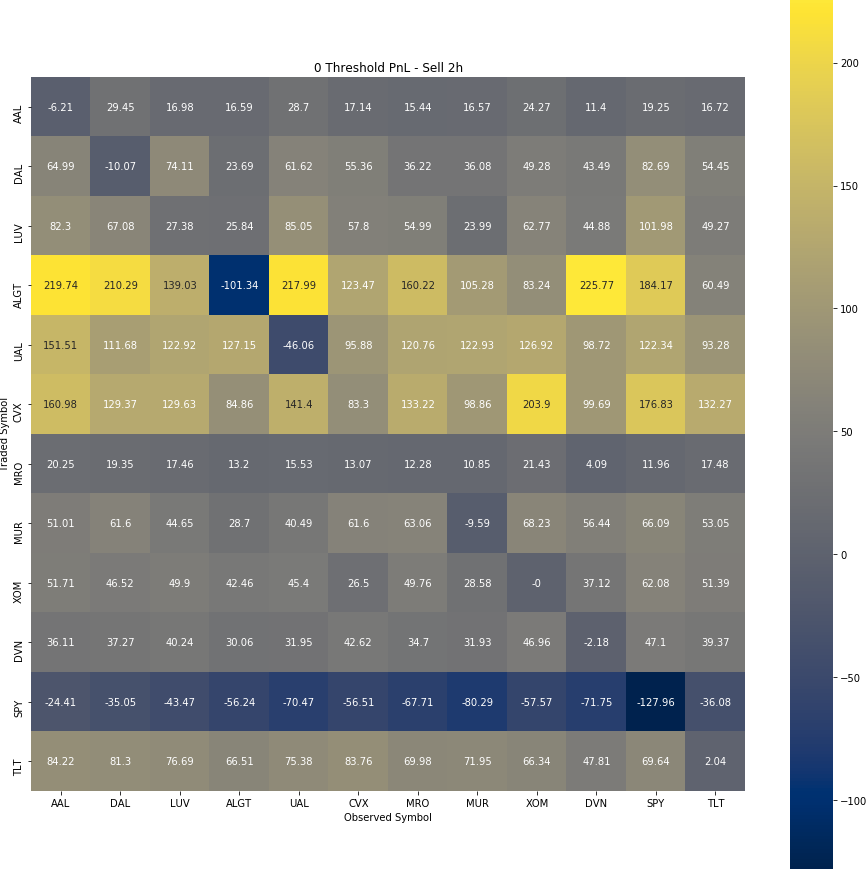
\includegraphics[width=.95\linewidth]{../Figures/pair_sell_pnl_2h.png}
    \caption{Sell Side PnL}
  \end{subfigure}
  \caption{2-Hour Markouts}
\end{figure}

\begin{figure}[h!]
  \centering
  \begin{subfigure}{.5\textwidth}
    \centering
    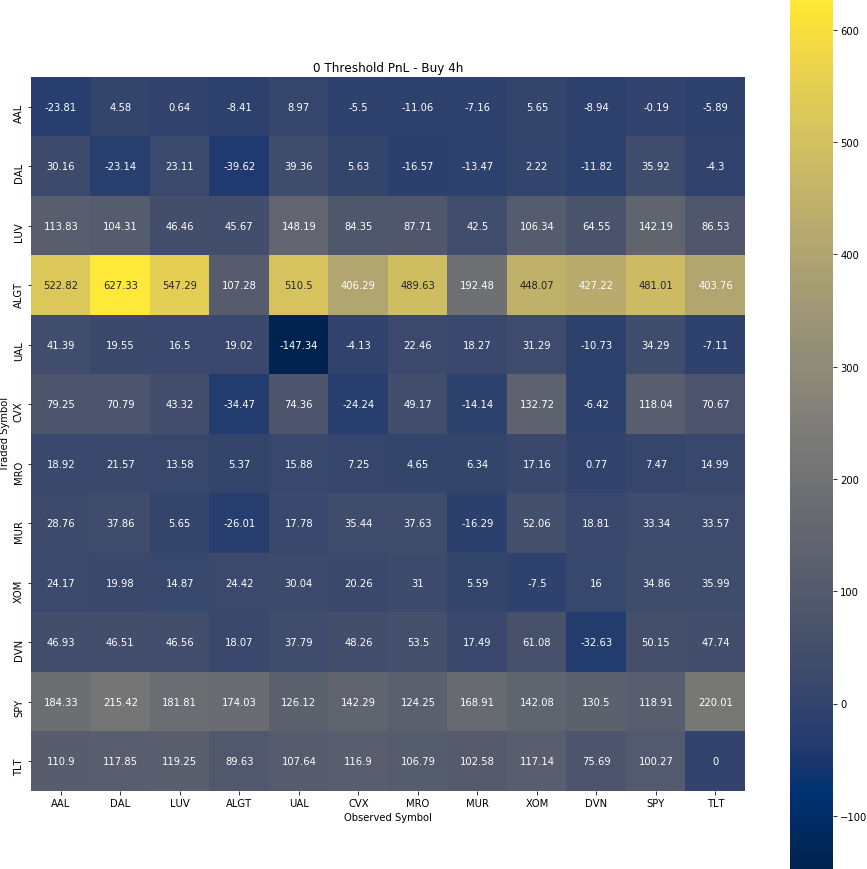
\includegraphics[width=.95\linewidth]{../Figures/pair_buy_pnl_4h.png}
    \caption{Buy Side PnL}
  \end{subfigure}%
  \begin{subfigure}{.5\textwidth}
    \centering
    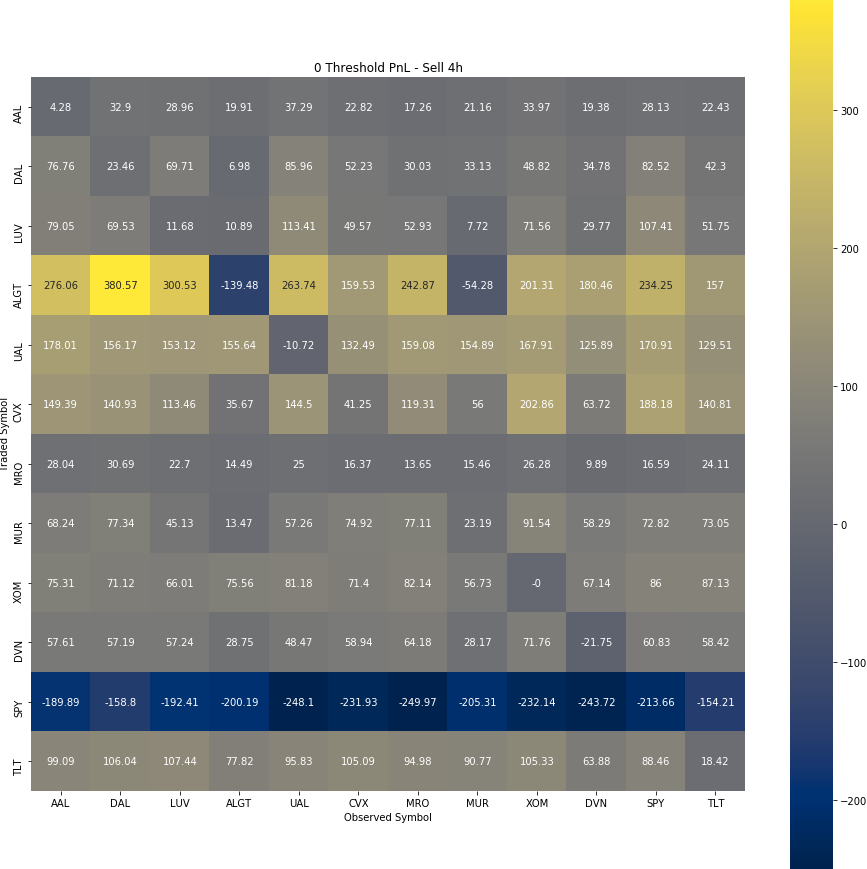
\includegraphics[width=.95\linewidth]{../Figures/pair_sell_pnl_4h.png}
    \caption{Sell Side PnL}
  \end{subfigure}
  \caption{4-Hour Markouts}
\end{figure}

\begin{figure}[h!]
  \centering
  \begin{subfigure}{.5\textwidth}
    \centering
    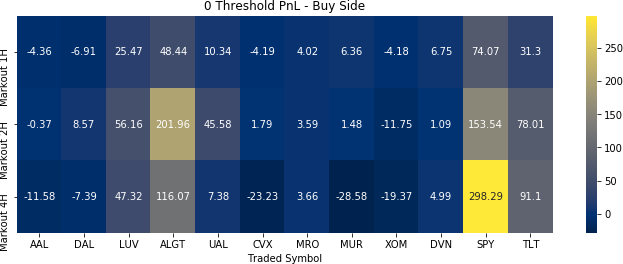
\includegraphics[width=.95\linewidth]{../Figures/basket_buy_pnl.png}
    \caption{Buy Side PnL}
  \end{subfigure}%
  \begin{subfigure}{.5\textwidth}
    \centering
    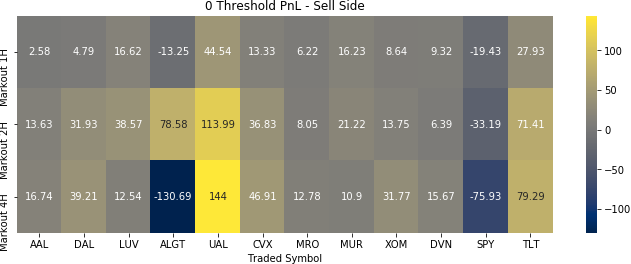
\includegraphics[width=.95\linewidth]{../Figures/basket_sell_pnl.png}
    \caption{Sell Side PnL}
  \end{subfigure}
  \caption{Basket Model PnL}
\end{figure}

\end{document}